%-------------------------------------------------------------------------------
%	NAME:	report.tex
%	AUTHOR: Connor Beardsmore - 15504319
%	LAST MOD: 01/04/17
%	PURPOSE:	AMI Assignment Report
%	REQUIRES:	NONE
%-------------------------------------------------------------------------------

\documentclass[]{article}
\usepackage[ margin=3cm ]{geometry}
\usepackage{graphicx}
\usepackage{fancyhdr}
\usepackage{float}
\usepackage{hyperref}
\usepackage{transparent}
\usepackage{pdfpages}
\usepackage[style=chicago-authordate,backend=biber]{biblatex}

\pagestyle{fancy}
\fancyhf{}
\lhead{Connor Beardsmore - 15504319}
\rhead{AMI300}
\lfoot{May 2017}
\rfoot{\thepage}

\pagenumbering{arabic}
\graphicspath{{./images/}}

\addbibresource{bib/references.bib}
\nocite{*}

%-------------------------------------------------------------------------------
\begin{document}
%-------------------------------------------------------------------------------
% OFFICIAL COVER PAGE

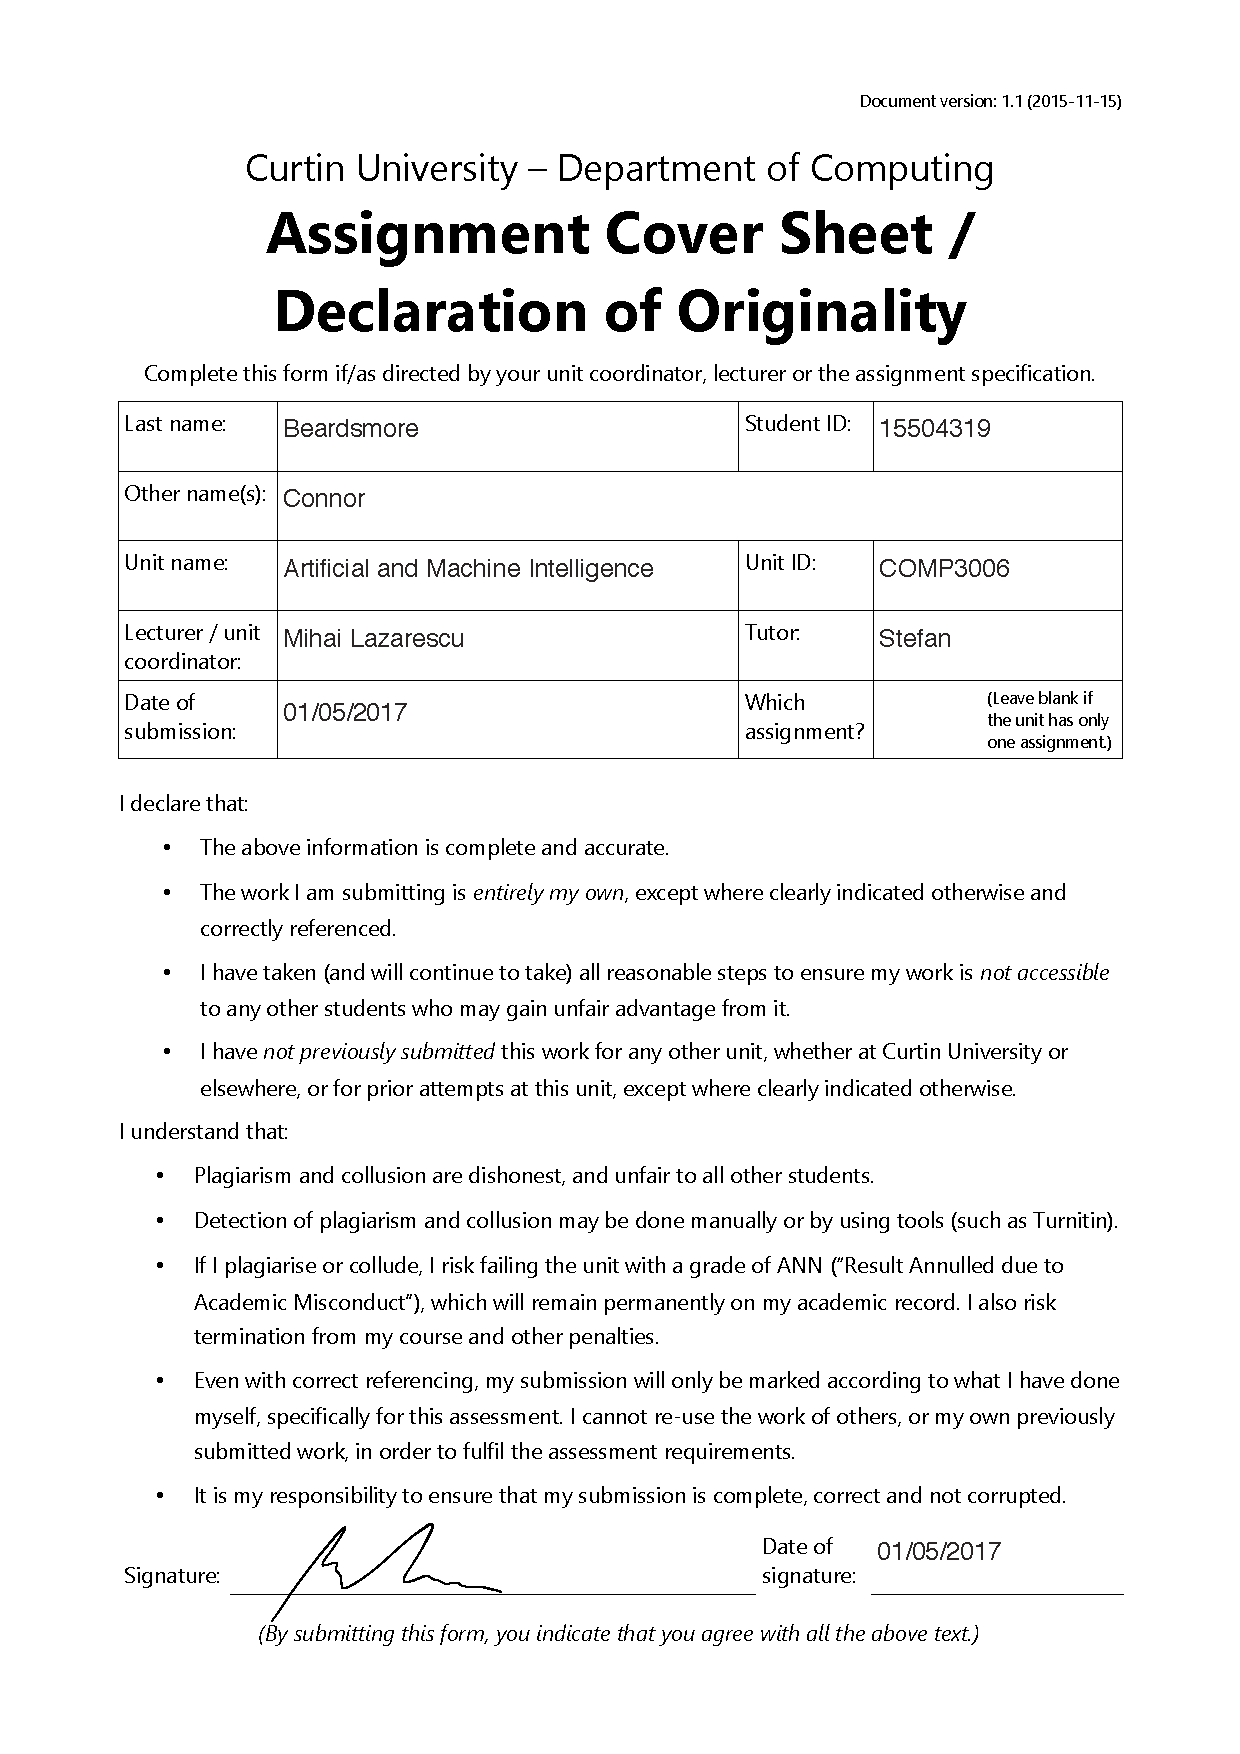
\includepdf[]{coverpage.pdf}
	
%-------------------------------------------------------------------------------
% TITLE PAGE

\begin{titlepage}
	\begin{center}
		\vspace*{1cm}
		\LARGE\textbf{AMI300 Report} \vspace{0.5cm}
		\break
	    Informed Beam and SMA* Search Implementations
		\vspace{1cm}
		\break
		\Large\textbf{Connor Beardsmore - 15504319} 
		\vspace{15cm}

		\normalsize
		Curtin University \\
		Science and Engineering \\
		Perth, Australia \\
	    May 2017
	    
	\end{center}
\end{titlepage}

%-------------------------------------------------------------------------------
% AFFINE CIPHER

\vspace*{-0.8cm}
\begin{center}
	\section*{Informed Beam Search}
\end{center}

\vspace*{0.8cm}
\subsection*{Design Decisions}

sdsdsdsd

\vspace*{0.8cm}
\subsection*{Problems and Bugs}

dsdsaddas

\pagebreak

\begin{center}
	\section*{Simplified Memory Limited A* Search}
\end{center}

\vspace*{0.8cm}
\subsection*{Design Decisions}

sdsdsdsd

\vspace*{0.8cm}
\subsection*{Problems and Bugs}

sdsdsdsad

%-------------------------------------------------------------------------------   
% REFERENCES

\break
\setlength\bibitemsep{4\itemsep}
\printbibliography[title={References}]

%-------------------------------------------------------------------------------
\end{document}   
%-------------------------------------------------------------------------------